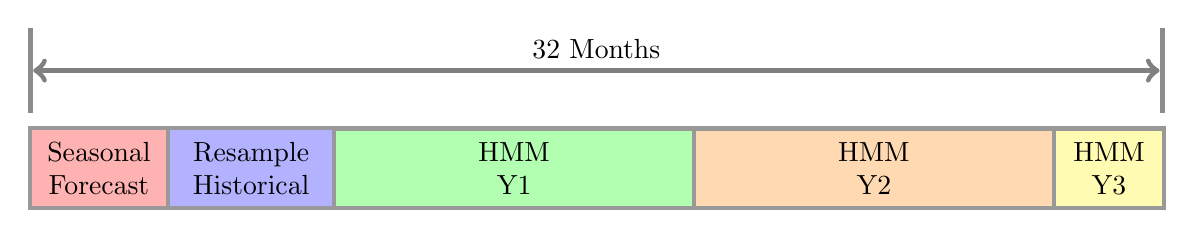
\begin{tikzpicture}[
rec/.style={
    rectangle,
    draw=gray!80,
    align=center,
    anchor=south west,
    inner sep = .5em,
    line width=1.5pt    
    },
line/.style={
    line width=1pt,
    draw=gray!90,
    text width=0pt,
    inner sep=0,
    text height = 3em,
    anchor = south west}
]
\node(seasonal) at (0,0) [rec,text width=4em,fill=red!30] {Seasonal Forecast};
\node(resample) [rec,text width=5em,fill=blue!30] at (5em,0) {Resample Historical};
\node(hmmy1) [rec,text width=12em,fill=green!30] at (11em,0) {HMM\\ Y1};
\node(hmmy2) [rec,text width=12em,fill=orange!30] at (24em,0) {HMM\\ Y2};
\node(hmmy3) [rec,text width=3em,fill=yellow!30] at (37em,0) {HMM\\ Y3};
\node(lleft) at (0,3.5em) [line] {};
\node(lright) [line,anchor=south] at (41em,3.5em) {};
\draw[<->,draw=gray,line width=2pt] (lleft) edge node[above] {32 Months} (lright) ;
\end{tikzpicture}